%\vspace{1.5pc}
\vspace{1.5pc}
%\section[State of the Art]{State of the Art}
\vspace{-1pc}
\section[Penelitian Terkait dan Tahapan Penelitian IOD]{Penelitian Terkait dan Tahapan Penelitian IOD}
\begin{spacing}{1.5}
	Berdasarkan hasil analisis data observasi selama 40 tahun (1958-1997), \citeA{Saji1999} menunjukkan suatu fenomena mode dipol di Samudera Hindia, yaitu pola variasi internal dengan suhu permukaan laut (\textit{sea surface temperature} (SST)) anomali yang rendah di sekitar Sumatra dan SST yang tinggi di sebelah barat Samudera Hindia, dengan angin dan presipitasi yang menyertainya. Keterkaitan spasial-temporal antara SST dan angin mengungkapkan keterkaitan yang kuat melalui medan presipitasi dan dinamika laut. Proses interaksi udara-laut ini unik dan melekat pada Samudera Hindia, dan terbukti independen dari fenomena El Nino (osilasi selatan). Penemuan mode dipol ini yang menjelaskan sekitar 12\% dari variasi SST di Samudera Hindia, dan pada tahun-tahun aktifnya juga menyebabkan curah hujan yang parah di Afrika Timur dan kekeringan di Indonesia. 
	
	\citeA{Liu2023} menemukan anomali salinitas positif yang signifikan di lapisan atas Samudra Hindia tropis pusat selama periode tertentu dan menganalisis kondisi atmosfer dan proses dinamika samudra yang terkait dengan peristiwa ini. \citeA{Chu2022} mempelajari dinamika variasi antartahunan arus khatulistiwa di Samudra Hindia dan mengukur efek dari mode iklim ENSO dan IOD pada arus. \citeA{Xing2022} mengeksplorasi respons arus laut khatulistiwa selama fase puncak IOD, yang memberikan umpan balik positif laut yang mendukung puncak IOD. \citeA{Zhang2021} meneliti Atlantic Nino dan dampaknya pada iklim regional dan global. Secara keseluruhan, studi-studi ini berkontribusi pada pemahaman kita tentang interaksi kompleks antara arus laut, kondisi atmosfer, dan variabilitas iklim di Samudra Hindia dan Atlantik.
	
	\citeA{Polonsky2021} mengkaji fitur pembentukan lapisan kritis di zona ekuator-tropika Samudra Hindia, dan bagaimana hal tersebut terkait dengan terbentuknya IOD. \citeA{Valsala2020} meneliti dampak IOD pada siklus karbon di atas laut dan variasinya di Samudra Hindia, dengan pengamatan biogeo kimia dan model sirkulasi biogeo kimia laut global. Mereka menemukan bahwa IOD menyebabkan variasi signifikan dalam pengeluaran CO2 dari laut ke udara di wilayah tenggara tropika Samudra Hindia karena dinamika upwelling dan anomali bergerak ke barat. \cite{Zhang2020} membedakan IOD dari pola tripole baru yang baru saja ditemukan, yang memiliki SSTAs positif (negatif) di atas wilayah tengah tropika (tenggara dan barat) Samudra Hindia..
\end{spacing}
\vspace{-1pc}
\section[Model Numerik dan Parameter]{Model Numerik dan Parameter}
\begin{spacing}{1.5}
	\par Dalam subbab ini, akan dibahas mengenai persamaan untuk parameter dan deskripsi tentang model numerik yang digunakan dalam penelitian ini.
	
	Model sirkulasi laut atau \textit{Ocean General Circulation Models} (OGCM) menggunakan persamaan Navier-Stokes untuk memodelkan fenomena fisis yang terjadi di lautan. Lautan adalah fluida yang dapat dijelaskan dengan baik dengan pendekatan persamaan-persamaan primitif, yaitu persamaan Navier-Stokes serta persamaan keadaan nonlinier yang menggabungkan dua parameter (temperatur dan salinitas) dengan kecepatan fluida, dan mempertimbangkan beberapa asumsi dan hipotesis \shortcite{madec_gurvan_2022_6334656}.
	
	Beberapa asumsi yang digunakan dalam persamaan Navier-Stokes diantaranya asumsi Boussinesq, asumsi hidrostatik, dan asumsi tak termampatkan (\textit{incompressibility}). Misalkan $\rho$ sebagai densitas in situ, $T$ sebagai temperatur potensial, $S$ sebagai salinitas, $p$ sebagai tekanan, $z$ sebagai koordinat vertikal, dan $g$ sebagai percepatan gravitasi. Asumsi yang digunakan dalam persamaan Navier-Stokes dapat dituliskan sebagai berikut.\\
	Asumsi Boussinesq
	\begin{equation}\label{eq:P1}
		\rho = \rho(T,S,p).
	\end{equation}
	Berdasarkan asumsi Boussinesq, pengaruh variasi densitas terhadap sistem diabaikan kecuali kontribusinya terhadap gaya apung.\\
	Asumsi hidrostatik
	\begin{equation}
		\frac{\partial p}{\partial z} = -\rho g.
	\end{equation}
	Berdasarkan asumsi hidrostatik, persamaan momentum vertikal direduksi menjadi persamaan kesetimbangan antara parameter gradien tekanan vertikal dan gaya apung.\\
	Asumsi tak termampatkan
	\begin{equation}
		\nabla \;.\; U =\frac{\partial u}{\partial x} + \frac{\partial v}{\partial y} + \frac{\partial w}{\partial z} = 0.
	\end{equation}	
	Berdasarkan asumsi tak termampatkan, persamaan 3-D divergensi untuk vektor kecepatan $U = (u,v,w)$ (dalam koordinat kartesius $(x,y,z)$) dianggap sama dengan 0.
	
	Selanjutnya misalkan $U = U_h + wk$ ($h$ adalah notasi vektor horizontal lokal di atas bidang $(i,j)$). Persamaan vektor invarian (invarian di bawah transformasi koordinat sehingga dapat diterapkan secara seragam dalam sistem koordinat lengkung ortogonal mana pun) dari persamaan primitif dalam sistem vektor $(i, j, k)$ dapat dituliskan dalam persamaan berikut \shortcite{madec_gurvan_2022_6334656}.\\
	Persamaan kesetimbangan momentum
	\begin{equation}\label{eq:P2}
		\begin{aligned}
			\frac{\partial U_h}{\partial t} = - \left[(\nabla \times U) \times U + \frac{1}{2}\nabla (U^2)\right]_h - f \; k \times U_h - \frac{1}{\rho_o}\nabla_h p + D^U + F^U.
		\end{aligned}
	\end{equation}
	Dalam Persamaan (\ref{eq:P2}) di atas, suku $(\nabla \times U) \times U + \frac{1}{2}\nabla (U^2)$ dapat ditulis sebagai $U\cdot \nabla U$ dan merupakan suku percepatan konvektif dari persamaan momentum. Suku $\nabla_h p$ merupakan gradien tekanan, $f = 2\Omega\; \cdot \;k$ merupakan percepatan Coriolis (dengan $\Omega$ adalah vector kecepatan sudut bumi), $D^U$ merupakan parameterisasi dari fisika skala kecil untuk momentum sedangkan $F^U$ merupakan suku gaya permukaan untuk momentum.\\
	Persamaan konservasi panas dan salinitas
	\begin{equation}\label{eq:P3}
		\begin{aligned}
			\frac{\partial T}{\partial t} &= - \nabla \; . \; (T\;U)  + D^T + F^T \\
			\frac{\partial S}{\partial t} &= - \nabla \; . \; (S\;U)  + D^S + F^S,
		\end{aligned}
	\end{equation}
	dengan operator $\nabla$ sebagai vektor turunan yang diperumum dalam arah $(i,j,k)$, parameter $D^T$ dan $D^S$ merupakan parameterisasi dari fisika skala kecil untuk temperatur dan salinitas sedangkan parameter $F^T$ dan $F^S$ merupakan suku gaya permukaan untuk temperatur dan salinitas. 
	
	Untuk parameter lainnya seperti kedalaman lapisan campuran atau \textit{mixed layer depth} (MLD), \textit{chlorophyll-a} (Chl-a), laju presipitasi, fluks air tawar, fluks panas bersih, dan tekanan angin dapat dituliskan sebagai berikut.
	
%	Dalam aplikasinya, persamaan Navier-Stokes tidak hanya digunakan untuk memodelkan laut, tapi juga merambah ke bidang pemodelan cuaca \shortcite{Rohli2021}, aliran air dalam pipa \shortcite{Ouchiha2012} dan aliran udara di sekitar sayap pesawat \shortcite{Tulus2019}. Dalam bentuk persamaan lengkap dan simplifikasi, persamaan ini juga dapat digunakan untuk mendesain kereta api \shortcite{Croquer2020}, pesawat terbang \shortcite{Chau2021}, dan mobil \shortcite{Ambarita2018}. Terdapat juga studi tentang aliran darah \shortcite{Gill2021}, desain stasiun pembangkit listrik \shortcite{Yang2019}, dan analisis polusi udara \shortcite{Issakhov2022}. 
	
\end{spacing}
\vspace{-1pc}
\section[\textit{Road Map }Penelitian]{\textit{Road Map} Penelitian}
\begin{spacing}{1.5}
	\textit{Road Map} penelitian ini dapat dilihat dalam Gambar \ref{fig:RM}
	\begin{figure}[H]
		\centering
		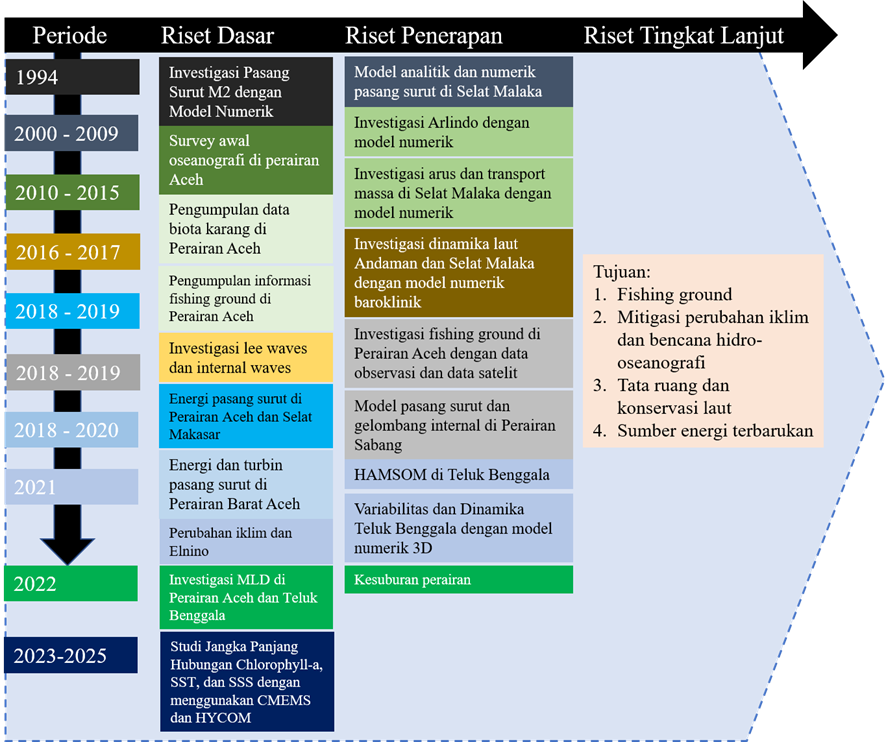
\includegraphics[width=12cm]{contents/Figures/Road_Map}
		\caption{Road Map Penelitian}
		\label{fig:RM}
	\end{figure}
	
\end{spacing}